%!TEX root=../GaugeCNNTheory.tex


\subsection{Isometries and their action on manifolds, bundles and fields}
\label{sec:isom_background}


\begin{figure}
    \centering
    \subcaptionbox{\small Action of different subgroups of the isometry group on fields.
        \label{fig:isom_egg_actions}}%
        [.6\linewidth][l]{
            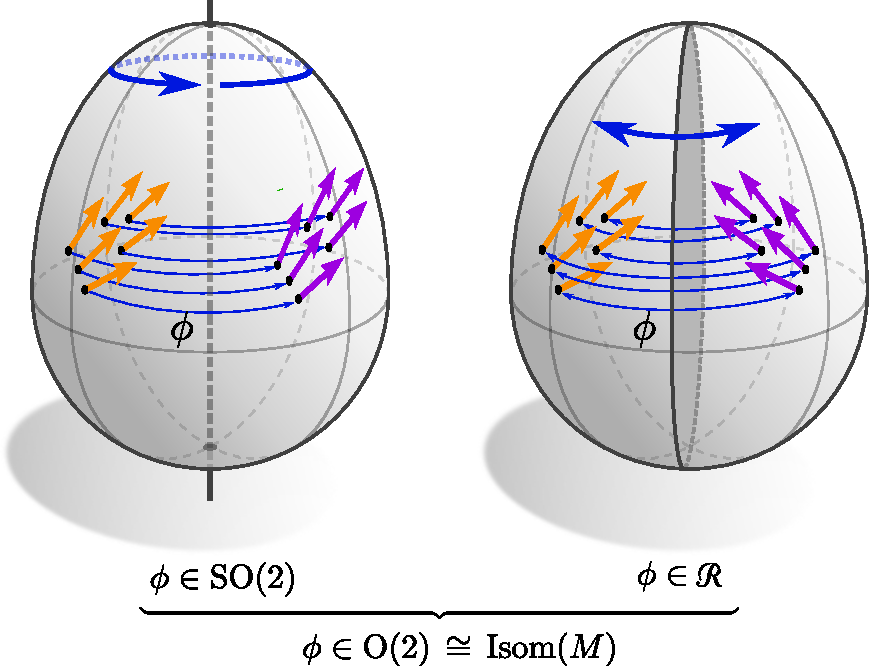
\includegraphics[width=.575\textwidth]{figures/isometry_egg_action.pdf}
        }
    \hfill
    \subcaptionbox{\small Orbits of the isometry group.
        \label{fig:isom_egg_orbits}}%
        [.3\linewidth][r]{
            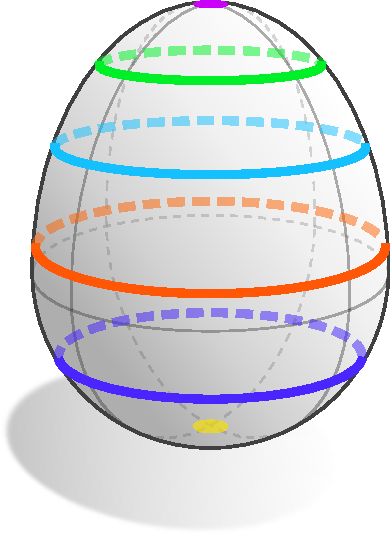
\includegraphics[width=.26\textwidth]{figures/isometry_egg_orbits.pdf}
            \hspace*{2ex}
            \vspace*{7.0ex}
        }
    \caption{\small
        Visualizations of the isometry group $\IsomM \cong \O2$ of an egg $M$, which we will use throughout this section to exemplify different concepts and constructions relating to isometries.
        Fig.~\ref{fig:isom_egg_actions} shows the action of the isometry group on (tangent or feature) vector fields.
        It can be thought of as consisting of the subgroups of rotations in $\SO2$ and reflections in $\Flip$.
        The action of the isometry group partitions the egg into orbits $\IsomM.p = \big\{\phi(p) \,\big|\, \phi\in\IsomM\big\}$ of points $p\in M$, shown in Fig.~\ref{fig:isom_egg_orbits} in different colors.
        Note that not all orbits are homeomorphic to each other -- the orbits at the poles are single points while any other orbit traces out a circle around the egg.
        The isometry group of the egg acts non-transitively on it, that is, not every point can be reached from any other point.
        A~kernel field transform is isometry equivariant if it commutes with the isometry action on feature fields.
        We show that isometry equivariance is guaranteed if and only if the kernel field is invariant under the action of isometries.
        This implies in particular that isometry equivariance require weight sharing along the isometry orbits; see Fig.~\ref{fig:isom_invariant_kernel_field_multiple_orbits}.
    }
    \label{fig:isom_egg_main}
\end{figure}


In this section we introduce most of the mathematical concepts required for our study of the isometry equivariance of kernel field transforms and $\GM$-convolutions.
After defining isometries in Section~\ref{sec:isometry_groups}, we discuss in Section~\ref{sec:isom_action_bundles} how they induce natural actions on tangent vectors and reference frames.
For structure groups $G<\O{d}$, not any isometry is compatible with any $G$-structure.
We define the subgroup $\IsomGM \leq \IsomM$ of those isometries which do act on (induce automorphisms of) a $G$-structure $\GM$ and their $G$-associated feature bundles.
While these constructions are kept coordinate free, Section~\ref{sec:isom_coordinatization} expresses the action of isometries on fiber bundles relative to local bundle trivializations.
In preparation for our investigation of isometry equivariant kernel field transforms later on, Section~\ref{sec:isom_expmap_transport} discusses how isometries commute with the exponential map and with parallel transporters, which allows to derive how isometries act on the transporter pullback $\Expspf$ of feature fields~$f$.
While staying mostly mathematical, we try to draw connections to the application wherever possible.


\subsubsection{Isometry groups}
\label{sec:isometry_groups}

A (global) \emph{isometry} $\phi: M \to \hat{M}$ is a diffeomorphism between Riemannian manifolds $(M,\eta)$ and $(\hat{M},\hat{\eta})$, which \emph{preserves the metric}.
In terms of the pushforward (differential) $\dphiTM: \TM \to T\mkern-1.5mu\hat{M}$ of tangent vectors, which we introduce in Appendix~\ref{apx:differentials_gradients_jacobians} and in Section~\ref{sec:isom_action_bundles} below, this statement is made precise by requiring that isometries satisfy
\begin{align}\label{eq:isometry_def}
    \eta_p(v,\, w)\ =\ \hat{\eta}_{\phi(p)}( \dphiTM v,\, \dphiTM w) \qquad \forall\ \ p\in M,\,\ v,w\in \TpM \,,
\end{align}
i.e. that they preserve distances and angles between tangent vectors.
Intuitively, an isometry is thought of as a distance preserving map between manifolds.
Note that the inverse of an isometry is necessarily an isometry as well.
Since isometries (and their inverses) respect the metric, they constitute the \emph{isomorphisms in the category of Riemannian manifolds}.


The set of all isometries $\phi: M \to M$ from a Riemannian manifold to itself, equipped with the usual function composition $\circ: (\phi_1, \phi_2) \mapsto \phi_1 \circ \phi_2$, defines a group, known as \emph{isometry group} $\IsomM$ of~$M$.
This group is the automorphism group of a Riemannian manifold, which contains all of its (metric) ``symmetries''.
It is a subgroup of the diffeomorphism group $\Diff(M)$ of~$M$.
The full isometry group might have non-trivial subgroups, which we will in the following denote by $\I \leq \IsomM$.
An example is given in Fig.~\ref{fig:isom_egg_actions}, which visualizes the isometry group $\IsomM \cong \O2$ of an egg.
The full isometry group splits (for instance) into the subgroups of rotations in $\I_1 \cong \SO2$ and reflections in $\I_2 \cong \Flip$.


In general, the isometry group of a manifold is non-transitive, that is, not every point of $M$ can be reached from any other point by its action.
The manifold is then partitioned into disjoint \emph{orbits}, visualized for the example of $M$ being an (Easter) egg in Fig.~\ref{fig:isom_egg_orbits}.
The isometry group of a manifold $M$ might be trivial, given that $M$ is sufficiently asymmetric.
In this case there might still exist non-trivial isometries between open subsets $U^{\widetilde{A}}$ and $U^A$ of $M$, restricted to which Eq.~\eqref{eq:isometry_def} holds.
Fig.~\ref{fig:suzanne_local_isometry} shows an example of a manifold which is globally asymmetric but has non-trivial isometries between local subsets of itself.
We will in the following only consider global isometries of~$M$, however, all concepts of the current Section~\ref{sec:isom_background} generalize in an obvious way to isometries between local subsets.
Without proof, we claim that the same holds for the isometry equivariance of any neural network operation which acts pointwise, for instance \onexones, nonlinearities or bias summation.
The equivariance of kernel field transforms with spatially extended kernels holds up to boundary effects.

\begin{SCfigure}
    \centering
    \hspace{1.ex}
    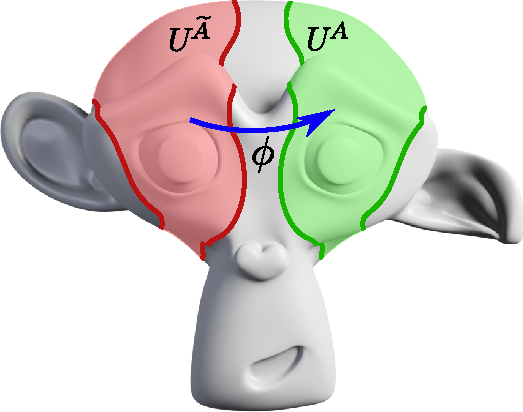
\includegraphics[width=.42\textwidth]{figures/suzanne_local_isometry.pdf}
    \hspace{2.ex}
    \captionsetup{width=.89\textwidth}
    \caption[]{\small
        An asymmetric manifold, whose \emph{global} isometry group is trivial.
        Since the asymmetry is limited to the ears and the mouth of
        ``\href{https://en.wikipedia.org/wiki/Blender_(software)\#Suzanne}{Suzanne}'',
        the monkey, there are non-trivial localized symmetries left.
        For instance, the smooth map ${\phi: U^{\widetilde{A}} \to U^A}$ between the red and green highlighted subsets preserves the metric locally.
        All concepts developed in Section~\ref{sec:isom_background} as well as the isometry equivariance of point-wise operations like \onexones\ generalize immediately to such isometries between local subsets. 
        The isometry equivariance of kernel field transforms with spatially extended kernels generalizes up to boundary effects.
        }
    \label{fig:suzanne_local_isometry}
\end{SCfigure}











\subsubsection{Isometry action on fiber bundles}
\label{sec:isom_action_bundles}

Isometries act naturally on tangent vectors in~$\TM$ and reference frames in~$\FM$ by ``carrying them along'' with the group action as visualized in Fig.~\ref{fig:isom_egg_actions}.
If an isometry is in addition compatible with the $G$-structure, that is, if it gives rise to an automorphism of~$\GM$, it furthermore acts on any associated $G$-bundle, in particular the feature vector bundles~$\A$.
We discuss these actions of isometries on the associated bundles and on feature fields in the following.



\paragraph{Isometry action on the tangent bundle \textit{TM}:}

Any isometry $\phi \in \IsomM$ gives rise to a \emph{pushforward}
\begin{align}
    \dphiTM: \TM \to \TM \,, \qquad \phi\in \IsomM
\end{align}
on the tangent bundle, which is just the differential of $\phi$ as introduced in Appendix~\ref{apx:differentials_gradients_jacobians}.
It can at each point $p \in M$ be thought of as a \emph{linear} approximation of $\phi$, which maps vectors $v \in \TpM$ to $\dphiTM(v) \in T_{\mkern-1mu\phi(p)}\mkern-2mu M$, that is, it satisfies
\begin{align}\label{eq:pushfwd_bundle_automorphism}
    \piTM \circ \dphiTM \,=\, \phi \circ \piTM.
\end{align}
As argued in Appendix~\ref{apx:differentials_gradients_jacobians}, the pushforward is invertible with $(\dphiTM)^{-1} = (\phi^{-1})_{\mkern-2mu*\mkern-1mu\scalebox{.55}{$,\mkern-2muT\mkern-3muM$}}$, for which we will unambiguously write $\dphiTMinv$.%
\footnote{
    The invertibility does not hold for pushforwards in general but only for those of diffeomorphisms and thus isometries.
}
The pushforward of an element $\phi$ of the isometry group is therefore seen to be an (isometric) vector bundle automorphism of $\TM$ over $\phi$, satisfying the following commutative diagram:
\begin{equation}\label{cd:pushforward_TM}
\begin{tikzcd}[column sep=70pt, row sep=40, font=\normalsize]
    \TM
        \arrow[r, shift left=2.5pt, "\dphiTM"]
        \arrow[d, "\piTM"']
    &
    \TM
        \arrow[d, "\piTM"]
        \arrow[l, shift left=2.5pt, "\dphiTMinv"]
    \\
    M
        \arrow[r, shift left=2.5pt, "\phi"]
    &
    M
        \arrow[l, shift left=2.5pt, "\phiinv"]
\end{tikzcd}
\end{equation}
By the \emph{definition of isometries}, their pushforward preserves distances and angles, that is, 
\begin{align}\label{eq:metric_pushfwd_isometry}
    \eta_{\phi(p)} \big(\dphiTM v,\, \dphiTM w\big) \,=\, \eta_p(v,w)
    \qquad\ \forall\ \ p\in M,\ \  v,w\in \TpM,\ \ \phi \in \IsomM .
\end{align}
More details about pushforwards between tangent bundles are easily found in the literature, for instance in~\cite{schullerGeometricalAnatomy2016}.



\paragraph{Isometry action on the frame bundle \textit{FM}:}
The pushforward on $\TM$ immediately induces a corresponding principal bundle automorphism $\dphiFM$ on $\FM$ by pushing forward the individual frame vectors:
\begin{align}\label{eq:pushforward_FM_def}
    \dphiFM\!: \FM \to \FM,\ \ \ 
    [e_i]_{i=1}^d \mapsto \dphiFM\big([e_i]_{i=1}^d\big) := \big[\dphiTM(e_i)\big]_{i=1}^d \,,
    \qquad \phi\in \IsomM
\end{align}
It maps frames in $\FpM$ for arbitrary $p\in M$ to frames at $F_{\mkern-1mu\phi(p)}\mkern-2mu M$, that is, $\piFM \circ \dphiFM = \phi \circ \piFM$.
To see this, let $[e_p]_{i=1}^d \in \FpM$, then $\phi\circ \piFM\big([e_i]_{i=1}^d\big) = \phi(p)$ and
$ \piFM \circ \dphiFM \big([e_i]_{i=1}^d\big)
= \piFM \pig(\big[ \dphiTM(e_i) \big]_{i=1}^d \pig)
= \piTM \circ \dphiTM (e_j)
= \phi \circ \piTM(e_j)
= \phi(p)$
for any $j=1,\dots,d$.
It can further be checked to be invertible with
$(\dphiFM)^{-1} = (\phi^{-1})_{\mkern-2mu*\mkern-1mu\scalebox{.55}{$,\mkern-2mu F\mkern-3muM$}}$,
again abbreviated by $\dphiFMinv$.
The \emph{left action} of the $\dphiFM$ on the frame bundle commutes with the \emph{right action} $\lhd$ on its fibers, that is, for arbitrary $g\in \GL{d}$ and $\phi \in \IsomM$ we have that:
\begin{alignat}{3}
\label{eq:dpsiFM_right_GL_equiv}
    \qquad
    \Big(\dphiFM \pig( [e_i]_{i=1}^d \pig)\Big) \lhd g
    \ &=\ \big[\dphiTM (e_i)\big]_{i=1}^d \lhd g
        \qquad\quad && \big( \text{\small def. of $\dphiFM$, Eq.~\eqref{eq:pushforward_FM_def}} \big) \notag \\
    \ &=\ \Big[\sum\nolimits_j \dphiTM (e_j)\, g_{ji} \Big]_{i=1}^d
        \qquad\quad && \big( \text{\small def. of $\lhd$, Eq.~\eqref{eq:rightaction_FM} } \big) \notag \\
    \ &=\ \Big[\dphiTM \Big(\sum\nolimits_je_j g_{ji}\Big) \Big]_{i=1}^d
        \qquad\quad && \big( \text{\small linearity of $\dphiTM$ } \big) \notag \\
    \ &=\ \dphiFM \Big(\Big[\sum\nolimits_je_j g_{ji}\Big] \Big)_{i=1}^d
        \qquad\quad && \big( \text{\small def. of $\dphiFM$, Eq.~\eqref{eq:pushforward_FM_def}} \big) \notag \\
    \ &=\ \dphiFM \Big( [e_i]_{i=1}^d \lhd g \Big)
        \qquad\quad && \big( \text{\small def. of $\lhd$, Eq.~\eqref{eq:rightaction_FM} } \big)
\end{alignat}
A gauge transformation of a frame at $p\in M$ by $g\in \GL{d}$, followed by a pushforward to $\phi(p)$, is therefore equal to a pushforward of the untransformed frame, followed by a gauge transformation by the same group element $g$ but at $\phi(p)$.
Different frames in the fiber $\FpM$ are hence mapped in such a way to frames at $F_{\mkern-1mu\phi(p)}\mkern-2mu M$ that their relative offset is preserved.
The derived properties of $\dphiFM$ are summarized by the statement that the diagram
\begin{equation}\label{eq:FM_isom_induced_automorphism}
\begin{tikzcd}[column sep=70pt, row sep=35, font=\normalsize]
    \FM
        \arrow[r, "\dphiFM"]
    &
    \FM
    \\
    \FM
        \arrow[r, "\dphiFM"]
        \arrow[d, "\piFM"']
        \arrow[u, "\lhd g"]
    &
    \FM
        \arrow[d, "\piFM"]
        \arrow[u, "\lhd g"']
    \\
    M
        \arrow[r, "\phi"']
    &
    M
\end{tikzcd}
\end{equation}
commutes for any $\phi\in\IsomM$ and any $g\in \GL{d}$.
Satisfying the commutativity of this diagram, the pushforward $\dphiFM$ on the frame bundle is identified as a \emph{principal bundle automorphism}%
\footnote{
    I.e. a principal bundle isomorphism from the frame bundle to itself; cf. Eq.~\ref{cd:principal_bundle_morphism}.
}
over $\phi$.

Note that the inverses, which are shown explicitly in the diagram~\eqref{cd:pushforward_TM}, are omitted to reduce clutter.






\paragraph{Isometry action on \textit{G}-structures \textit{GM}:}

As $G$-structures are principal subbundles of the frame bundle, one can consider the restriction of the domain of the pushforward on~$\FM$ to~$\GM$, that is,
\begin{align}
    \dphiFM \mkern-2mu \big|_{\scalebox{.58}{$\GM$}} :\ \GM \to \FM \,, \qquad \phi\in \IsomM \,.
\end{align}
It is hereby necessary to keep the full frame bundle~$\FM$ as codomain since there is in general no guarantee that frames in~$\GpM$ are mapped to frames of $\GphipM$ but only to $\FphipM$.
\begin{figure}
    \centering
    \subcaptionbox{Canonical $\{e\}$-structure of $\R^2$
        \label{fig:frame_field_automorphism_1}}%
        [.49\linewidth][l]{
            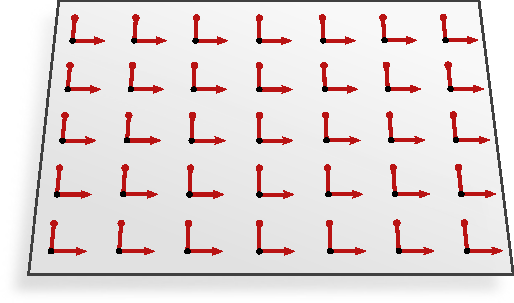
\includegraphics[width=.46\textwidth]{figures/frame_field_isom_equiv_1.pdf}
        }
    \subcaptionbox{An alternative $\{e\}$-structure on $\R^2$
        \label{fig:frame_field_automorphism_2}}%
        [.49\linewidth][l]{
            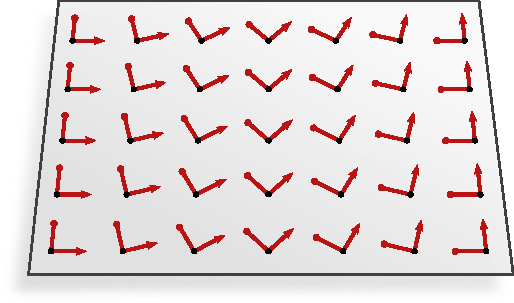
\includegraphics[width=.46\textwidth]{figures/frame_field_isom_equiv_2.pdf}
        }
    \caption[]{\small
        Two specific choices of $\{e\}$-structures (global frame fields) $\eM$ on $M = \R^2$, which we use to visualize the concept of \emph{$G$-structure preserving isometries}.
        The full isometry group of~$M$ is the Euclidean group~$\IsomM=\E2$, consisting of translations, rotations and reflections.
        Fig.~\ref{fig:frame_field_automorphism_1} shows the canonical $\{e\}$-structure of $\R^2$, which is invariant under translations but not under rotations or reflections.
        More abstractly stated, translations make up the subgroup $\IsomeM = \Trans_2 := (\R^2,+)$ of isometries that induce automorphisms of $\eM$.
        In contrast, rotations or reflections map frames in $\epM$ to frames in $\FphipM$ but fail to send them to~$\ephipM$.
        They do therefore not induce automorphisms of the $\{e\}$-structure and are not part of $\IsomeM$.
        Group actions of such isometries on~$\eM$ or any of its $\{e\}$-associated bundles \emph{are not defined}.
        Fig.~\ref{fig:frame_field_automorphism_2} shows an alternative choice of $\{e\}$-structure on $M = \R^2$ (or $M=\Euc_2$), which is only invariant under translations in the ``up-down'' direction, i.e. $\IsomeM \cong \Trans_1 = (\R,+)$.
        The examples in Figs.~\ref{fig:frame_field_automorphism_1} and~\ref{fig:frame_field_automorphism_2} exemplify that the $G$-structure automorphisms do not only depend on the structure group $G$ but on the particular choice of $G$-structure~$\GM$.
        The general case for $G$ being non-trivial is harder to visualize since $\GpM$ will then not be a single frame but a set of frames.
        }
    \label{fig:frame_field_automorphism}
\end{figure}
Since $G$-structures are in general not closed under the action of isometries on~$\FM$, it might be \emph{impossible} to define a group action of the full isometry group on~$\GM$ or any other associated $G$-bundle.
To remedy this shortcoming, we will in the following consider the subgroup of those isometries that respect the $G$-structure, i.e. which map preferred frames in~$\GM$ to frames in~$\GM$.
\begin{dfn}[$G$-structure preserving isometries]
\label{dfn:IsomGM}
    Given a $G$-structure $\GM$, we define the corresponding subgroup of $G$-structure preserving isometries $\IsomGM$ as:
    \begin{align}\label{eq:isomGM_def}
        \IsomGM\ :=\ \big\{ \phi \in \IsomM \,\big|\, \dphiFM(\GpM) = \GphipM\ \ \ \forall p \in M \big\} \ \leq\ \IsomM
    \end{align}
\end{dfn}
For such isometries, we define the induced action on~$\GM$ as
\begin{align}
    \dphiGM\, :=\, \dphiFM \mkern-2mu \big|_{\scalebox{.58}{$\GM$}} \,:\ \GM \to \GM \,, \qquad \phi\in \IsomGM \,.
\end{align}
Such defined actions for $\phi \in \IsomGM$ are \emph{$G$-structure automorphisms}, that is, they make the following diagram commute for any $g\in G$ (which follows by restricting Eq~\eqref{eq:FM_isom_induced_automorphism} from $\FM$ to $\GM$ and $\GL{d}$ to $G$):
\begin{equation}\label{cd:isom_induced_GM_automorphism}
\begin{tikzcd}[column sep=70pt, row sep=35, font=\normalsize]
    \GM
        \arrow[r, "\dphiGM"]
    &
    \GM
    \\
    \GM
        \arrow[r, "\dphiGM"]
        \arrow[d, "\piGM"']
        \arrow[u, "\lhd g"]
    &
    \GM
        \arrow[d, "\piGM"]
        \arrow[u, "\lhd g"']
    \\
    M
        \arrow[r, "\phi"']
    &
    M
\end{tikzcd}
\end{equation}
Fig.~\ref{fig:frame_field_automorphism} shows two examples of $\{e\}$-structures on $M=\R^2$, i.e. global frame fields.
From these examples it is apparent that the subgroups $\IsomGM$ do really depend on the particular choice of $G$-structure $\GM$, not only on the structure group~$G$.
In Fig.~\ref{fig:SO2_structure_SE2} we visualize an $\SO2$-structure on $M=\R^2$.
Its isometry group $\IsomSOM = \SE2$ is larger than those of the $\{e\}$-structures in Fig.~\ref{fig:frame_field_automorphism}.
An $\SO2$-structure on the sphere $S^2$, which is preserved by all rotations $\IsomSOM = \SO3$, is shown in Fig.~\ref{fig:SO2_structure_SE2}.


For specific choices of structure groups $G$ it is possible to make more general statements about which isometries are contained in the subgroup $\IsomGM$.
Most importantly, for orthonormal structure groups $G=\O{d}$ (which are compatible with $\eta$) \emph{any} isometry will induce an automorphism of~$\OM$, that is, one always has $\IsomOM = \IsomM \,.$
To prove this claim, let $[e_i]_{i=1}^d \in \OpM \subset \FpM$ be an orthonormal frame, which is by an arbitrary isometry $\phi \in \IsomM$ being sent to $\dphiFM \big|_{\scalebox{.58}{$\OM$}} [e_i]_{i=1}^d = \big[\dphiTM e_i\big]_{i=1}^d$; see Eq.~\eqref{eq:pushforward_FM_def}.
Applying Eq.~\eqref{eq:metric_pushfwd_isometry} to the individual axes of the pushforward frame yields
\begin{align}\label{eq:isom_orthonormal_to_orthonormal_frames}
    \eta\big( \dphiTM e_i, \dphiTM e_j \big) \,=\, \eta(e_i, e_j) \,=\, \delta_{ij}\ \quad\ \forall\ \ i,j \in 1,\dots,d \,,
\end{align}
which implies the orthonormality of of the pushforward frame $\dphiFM \big|_{\scalebox{.58}{$\OM$}} [e_i]_{i=1}^d \in \OphipM$ and therefore allows to define $\dphiOM := \dphiFM \big|_{\scalebox{.58}{$\OM$}}$ for any $\phi \in \IsomM$.
More generally, this result implies:
\begin{align}\label{eq:isomM_isomOM}
    \IsomGM = \IsomM \quad \ \forall\ G \geq \O{d}
\end{align}
It is similarly possible to show
\begin{align}\label{eq:isomplusM_isomSOM}
    \IsomSOM = \IsomplusM \,,
\end{align}
that is, that any orientation preserving isometry in $\IsomplusM$ induces an automorphism of an $\SO{d}$-structure $\SOM$.
Note that these statements all depend only on the structure group~$G$ but are independent from the specific choice of $G$-structure.
This is ultimately a result of only considering isometries, which are adapted to $\O{d}$-structures by definition, instead of considering more general diffeomorphisms.
As mentioned before, the subgroup $\IsomGM$ \emph{does} in general depend on the specific choice of $G$-structure $\GM$, not only the structure group~$G$.


\begin{figure}
    \centering
    \subcaptionbox{$\SE2$-invariant $\SO2$-structure $\SOM$ over $M = \R^2$.
        \label{fig:SO2_structure_SE2}}%
        [.5\linewidth][l]{
            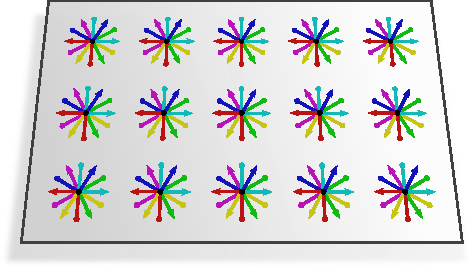
\includegraphics[width=.5\textwidth]{figures/SO2_structure_SE2.pdf}
            \rule{0pt}{20pt}
        }
    \subcaptionbox{$\SO3$-invariant $\SO2$-structure $\SOM$ over $M = S^2$\!\!.
        \label{fig:SO2_structure_SO3}}%
        [.48\linewidth][l]{
            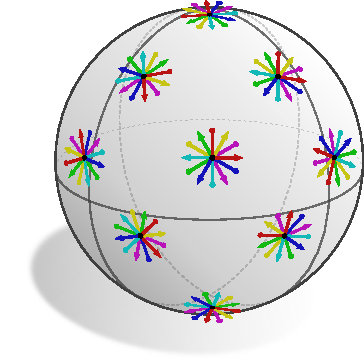
\includegraphics[width=.4\textwidth]{figures/SO2_structure_SO3.pdf}
        }
    \caption[]{\small
        Two examples of $\SO2$-structures $\SOM$ over the plane $M = \R^2$ and the sphere $M = S^2$.
        For ${M = \R^2}$, shown in Fig.~\ref{fig:SO2_structure_SE2}, the $\SO2$-structure is invariant under translations and rotations.
        As it consists only of right-handed frames (mind the arrow tips on the first and the circle tips on the second frame axes) it is not invariant under reflections.
        The isometries which preserve $\SOM$ therefore form the group $\IsomSOM = \SE2$, which is a subgroup of the full isometry group $\IsomM = \E2$.
        In the case of $M = S^2$, shown in Fig.~\ref{fig:SO2_structure_SO3}, the $\SO2$-structure is invariant under rotations but not under reflections.
        The $\SO2$-structure automorphisms are here $\IsomSOM = \SO3$ while the full isometry group is $\IsomM = \O3$.
        }
    \label{fig:SO2_structures_SE2_SO3}
\end{figure}















\paragraph{Isometry action on associated vector bundles $\A$:}
From the pushforward of isometries in $\IsomGM$ on $\GM$ one can construct a pushforward $\dphiA$ on any $G$-associated vector bundle $\A = (\GM\times\R^c)/\!\sim_{\!\rho}$ by defining
\begin{align}\label{eq:pushforward_A_def}
    \dphiA\!: \A \to \A,\ \ \
    \pig[[e_i]_{i=1}^d,\, \mathscr{f}\pig]
    \mapsto \dphiA\!\Big(\! \pig[[e_i]_{i=1}^d,\, \mathscr{f}\pig] \!\Big)
    := \Big[\dphiGM \big([e_i]_{i=1}^d \big),\, \mathscr{f}\Big] \,,
    \qquad \phi \in \IsomGM \,.
\end{align}
This action is well defined since the construction is by the right $G$-equivariance of $\dphiGM$ in Eq.~\eqref{cd:isom_induced_GM_automorphism} independent from the chosen representative of the equivalence class.
Similar to before, one has $\piA\mkern2mu\circ\mkern2mu \dphiA = \phi\mkern2mu \circ\mkern2mu \piA$, that is, $\dphiA$ maps feature vectors at $\A_p$ to feature vectors at $\A_{\phi(p)}$, which can be checked by acting on a feature vector and using the corresponding property of $\dphiGM$.
Since $\dphiA$ is defined by the action of $\dphiGM$ on the first factor in $(\GM\times\R^c)/\!\sim_{\!\rho}$\,, it does not interfere with linear combinations which act on the second factor as defined in Eq.~\eqref{eq:associated_bdl_linear_combination}.
This implies that the pushforward on associated bundles maps linearly between their fibers.
The invertibility of $\dphiA$ follows from the invertibility of $\dphiGM$ such that one again gets $(\dphiA)^{-1} = (\phi^{-1})_{\mkern-2mu*\mkern-1mu\scalebox{.55}{$,\mkern-2mu \A$}}$, which we write as $\dphiAinv$.
These properties, together with the fact that $\dphiGM \in \Aut(\GM)$ is in particular a principal bundle automorphism, identify $\dphiA$ as an \emph{associated vector bundle automorphism}, satisfying the following commutative diagram:
\begin{equation}\label{cd:associated_bdl_automorphism}
\begin{tikzcd}[column sep=70pt, row sep=35, font=\normalsize]
    \A
        \arrow[r, "\dphiA"]
        \arrow[d, "\piA"']
    &
    \A
        \arrow[d, "\piA"]
    \\
    M
        \arrow[r, "\phi"']
    &
    M
\end{tikzcd}
\end{equation}

The associated bundle resulting from the specific choices of $\rho(g)=g$ as group representation and $\R^d$ as typical fiber is via the bundle morphism $\chi:(\GM\times\R^d)/\!\!\sim\; \to \TM$ from Eq.~\eqref{eq:A_TM_isomorphism} isomorphic to the tangent bundle $\TM$ (as $G$-bundle).
Our definition of pushforwards on associated $G$-bundles is consistent with this identification since $\chi\circ\dphiA = \dphiTM\circ\chi$.
To see this, let $\big[[e_i]_{i=1}^d,\, \mathscr{v}\big] \in (\GM\times\R^d)/\!\!\sim\;$ be an element of the isomorphic associated bundle that is mapped to $\chi\big(\big[ [e_i]_{i=1}^d,\, \mathscr{v} \big]\big) = \sum_i e_i \mathscr{v}_i$.
Then we have
${\chi \circ \dphiA \big( \big[[e_i]_{i=1}^d,\, \mathscr{v}\big] \big)}
 = \chi \big( \big[[\dphiTM(e_i)]_{i=1}^d,\, \mathscr{v}\big] \big)
 = \sum_i \dphiTM(e_i) \mathscr{v}_i
 = \dphiTM \big(\sum_i e_i \mathscr{v}_i \big)
 = \dphiTM \circ \chi\big(\big[ [e_i]_{i=1}^d,\, \mathscr{v} \big]\big) \,,
$
which shows the consistency of the definitions.


As an associated bundle, the pushforward $\dphiHom$ on the homomorphism bundle $\Hom(\Ain,\Aout) \cong {(\GM\times\R^{\cout\times\cin})/\!\sim_{\!\rhoHom}}$ is specified by Eq.~\eqref{eq:pushforward_A_def} as well.
However, we will later on require an expression of $\dphiHom$ in terms of the pushforwards $\dphiAin$ and $\dphiAout$ of $\Ain$ and $\Aout$, respectively, which we will shortly derive here.
For that purpose, let $H\in \Hom(\Ain|_p,\Aout|_p)$ be a homomorphism at $p$ and $f_p\in \Ainp$ be a feature vector at~$p$.
Then $H(f_p)$ is by definition a feature vector in $\Aoutp$.
In order to be consistently defined, the pushforward of the input feature vector $f_p$, being acted on by the pushforward of the homomorphism $H$, needs to agree with the pushforward of the output feature vector $H(f_p)$.
This implies
\begin{align}
    \dphiAout \big[ H(f_p) \big]
    \ =\  \big[ \dphiAout H\, \dphiAin^{-1} \big] \big( \dphiAin f_p \big)
    \ =:\ \big[ \dphiHom H \big] \big( \dphiAin f_p \big) \,,
\end{align}
where we defined the pushforward on the homomorphism bundle as:
\begin{align}\label{eq:pushforward_Hom_def}
    \dphiHom\!: \Hom(\Ain,\Aout) \to \Hom(\Ain,\Aout), \quad
    H \mapsto
    \dphiAout H\, \dphiAininv \,,
    \qquad\ \phi \in \IsomGM
\end{align}
Note that the composition of an element $H\in \Hom(\Ain,\Aout)$ with $\dphiAout$ on the left and with $\dphiAininv$ on the right mirrors the style of Eq.~\eqref{eq:Hom_bdl_triv_ptwise}.





\paragraph{Isometry action on feature fields:}
The actions of isometries in $\IsomGM$ on the associated bundles give rise to actions on their sections, in particular on feature fields.
This pushforward of sections is defined as follows:
\begin{dfn}[Isometry pushforward of feature field:]
\label{dfn:isometry_pushforward}
    Let $f\in \Gamma(\A)$ be a feature field and let $\phi\in \IsomGM$ be a $G$-structure preserving isometry.
    The isometry acts on the feature field via the \emph{pushforward}%
    \footnote{
        Note the similarity of this definition to that of the \emph{induced representation}, which is the group action w.r.t. which steerable CNNs are designed to be equivariant~\cite{Cohen2017-STEER,3d_steerableCNNs,Weiler2019_E2CNN}.
    }
    \begin{align}\label{eq:pushforward_section_A}
        \rhd\!:\ \IsomGM \mkern-2mu\times\mkern2mu \Gamma(\A) \to \Gamma(\A), \quad
        (\phi,f) \mapsto \phi\rhd\!f \,:=\, \dphiA\! \circ f \circ \phiinv \,.
    \end{align}
    In terms of a commutative diagram, this definition is visualized as:
    \begin{equation}\label{cd:pushforward_section_A}
    \qquad\qquad
    \begin{tikzcd}[column sep=70pt, row sep=35, font=\normalsize]
        \A
            \arrow[r, "\dphiA"]
        &
        \A
        \\
        M
            \arrow[r, "\phi"']
            \arrow[u, "f\ "]
        &
        M
            \arrow[u, "\ \phi\rhd\!f\ :=\: \dphiA \!\circ\mkern-2mu f \circ \phiinv"']
    \end{tikzcd}
    \end{equation}
\end{dfn}
Intuitively, this definition states that the pushforward section $\phi\rhd\!f$, evaluated at $p\in M$, returns the feature vector of $f$ from $\phi^{-1}(p)$, pushed forward to $p$ via $\dphiA$.
Note that such pushforwards do indeed yield well defined sections, which satisfy
\begin{align}
    \piA \circ (\phi\rhd \!f)
    \ &=\ \piA \circ \dphiA\! \circ f \circ \phiinv \notag \\
    \ &=\ \phi \circ \piA \circ f \circ \phiinv \notag \\
    \ &=\ \phi \circ \id_M \circ \phiinv \notag \\
    \ &=\ \id_M
\end{align}
as required by Eq.~\eqref{cd:section_proj_idM}.
Fig.~\ref{fig:isom_egg_actions} visualizes the action of isometries on fields.
The action of isometries on the transporter pullback $\Expspf$ of a fields~$f$ is derived in Section~\ref{sec:isom_expmap_transport} below.

















\subsubsection{Isometry action in local coordinates}
\label{sec:isom_coordinatization}

Most of the derivations on the isometry equivariance of kernel field transforms in Sections~\ref{sec:isometry_equivariance} and~\ref{sec:quotient_kernel_fields} will be kept in a coordinate free setting.
However, since $\GM$-convolutions are defined relative to a choice of $G$-atlases of the associated bundles, the investigation of their isometry equivariance will require us to study coordinate expressions of the isometry pushforwards $\dphiTM$, $\dphiFM$, $\dphiGM$ and $\dphiA$ relative to local bundle trivializations.
Coordinate expressions of the isometry action are furthermore useful in numerical implementations, which are necessarily encoding feature fields relative to fields of reference frames.

In the following, we assume gauges $\PsiTM^{\widetilde{A}}$ and $\PsiTM^A$ on neighborhoods $U^{\widetilde{A}}$ of $p$ and $U^A$ of $\phi(p)$ to be given.
For convenience, let $U^A = \phi\big(U^{\widetilde{A}}\big)$ coincide with the image of $U^{\widetilde{A}}$ under the isometry, which is always possible without losing generality.




\paragraph{Pushforward on \textit{TM} in coordinates:}
Recall that the pushforward on the tangent bundle is a linear map from vectors $v\in \TpM$ to vectors $\dphiTM v \in \TphipM$.
Relative to the given gauges, the pushforward is therefore coordinatized by a field of matrices%
\footnote{
    Given charts
    $x^{\widetilde{A}}: U^{\widetilde{A}} \to x^{\widetilde{A}}\big(U^{\widetilde{A}}\big) \subseteq \R^d$
    and
    $x^A: U^A \to x^A\big(U^A\big) \subseteq \R^d$
    of $M$, an isometry $\phi$ can be locally represented by a map
    $x^A \circ \phi \circ \big(x^{\widetilde{A}}\big)^{\mkern-1mu-1}\!: x^{\widetilde{A}}\big(U^{\widetilde{A}}\big) \to x^A\big(U^A\big)$
    between coordinates.
    For the special case that the gauges at $p$ and $\phi(p)$ correspond to the coordinate bases of those charts, $g_\phi^{A\widetilde{A}}$ is simply given by the \emph{Jacobian} of $x^A \circ \phi \circ \big(x^{\widetilde{A}}\big)^{\mkern-1mu-1}$.
}
\begin{align}\label{eq:pushforward_TM_coord}
    g_\phi^{A\widetilde{A}}\!: U^{\widetilde{A}} \to \GL{d},\ \ \ 
    p \mapsto g_\phi^{A\widetilde{A}}(p) := \psiTMphip^A \mkern-2mu\circ \dphiTM \mkern-2mu\circ \big(\psiTMp^{\widetilde{A}}\big)^{-1}
    , \quad\ \ \phi \in \IsomM \,,
\end{align}
which transforms between the corresponding numerical coefficients $\psiTMp^{\widetilde{A}}(v)$ of $v$ at $p$ and $\psiTMphip^A(\dphiTM v) = g_\phi^{A\widetilde{A}}(p) \psiTMp^{\widetilde{A}}(v)$ of $\dphiTM v$ at $\phi(p)$.
More precisely, $g_\phi^{A\widetilde{A}}$ takes values in the subgroup $\langle\, G\cup\O{d} \,\rangle$ of $\GL{d}$, which is generated by the elements of $\O{d}$ (due to $\dphiTM$ preserving the metric) and $G$ (since the transition functions might form a supergroup of $\O{d}$).
The definition of the pushforward in local coordinates is visualized by the following commutative diagram:
\begin{equation}\label{cd:pushforward_TM_coord}
    \begin{tikzcd}[row sep=4.em, column sep=5em]
        \R^d
            \arrow[rrr, pos=.5, rounded corners, to path={ 
                    -- ([yshift=-3.5ex]\tikztostart.south) 
                    --node[below]{\small$
                        g_\phi^{A\widetilde{A}}(p) \mkern2mu\cdot
                        $} ([yshift=-3.5ex]\tikztotarget.south) 
                    -- (\tikztotarget.south)
                    }]
        &
        \TpM
            \arrow[l, "\psiTMp^{\widetilde{A}}"']
            \arrow[r, "\dphiTM"]
        &
        \TphipM
            \arrow[r, "\psiTMphip^A"]
        &
        \R^d
    \end{tikzcd}
\end{equation}
Fig.~\ref{fig:pushforward_vector_components} gives a graphical interpretation of the pushforward in coordinates.


\paragraph{Pushforward on \textit{FM} in coordinates:}
The coordinatization of the pushforward on the frame bundle is defined in analogy to Eq.~\eqref{eq:pushforward_TM_coord}.
It turns out to be given by the left action of the same group element $g_\phi^{A\widetilde{A}}$ on trivialized frames as shown in the commutative diagram below:
\begin{equation}\label{eq:pushforward_FM_coord}
    \begin{tikzcd}[row sep=4.em, column sep=5em]
        \GL{d}
            \arrow[rrr, pos=.5, rounded corners, to path={ 
                    -- ([yshift=-3.5ex]\tikztostart.south) 
                    --node[below]{\small$
                        g_\phi^{A\widetilde{A}}(p) \mkern2mu\cdot
                        $} ([yshift=-3.5ex]\tikztotarget.south) 
                    -- (\tikztotarget.south)
                    }]
        &
        \FpM
            \arrow[l, "\psiFMp^{\widetilde{A}}"']
            \arrow[r, "\dphiFM"]
        &
        \FphipM
            \arrow[r, "\psiFMphip^A"]
        &
        \GL{d}
    \end{tikzcd}
\end{equation}
To prove this claim, we compute the action on a trivialized frame, given by a matrix $h \in \GL{d}$ whose $i$-th column $h_{:,i}$ represents the $i$-th frame vector:
\begin{alignat}{3}
    \qquad\qquad
       & \Big[ \psiFMphip^A \circ \dphiFM \circ \big(\psiFMp^{\widetilde{A}}\big)^{-1} \Big](h) \notag \\
    =\ & \Big[ \psiFMphip^A \circ \dphiFM \Big] \!\Big( \!\Big( \big(\psiTMp^{\widetilde{A}}\big)^{-1} (h_{:,i})\Big)_{i=1}^d \Big)
        \qquad\quad && \big( \text{\small def. of $\psiFMp^{\widetilde{A}}$, Eq.~\eqref{eq:trivialization_FM_p} } \big) \notag \\
    =\ & \psiFMphip^A \!\Big( \!\Big( \dphiTM \circ \big(\psiTMp^{\widetilde{A}}\big)^{-1} (h_{:,i})\Big)_{i=1}^d \Big)
        \qquad\quad && \big( \text{\small def. of $\dphiFM$, Eq.~\eqref{eq:pushforward_FM_def} } \big) \notag \\
    =\ & \Big( \!\Big( \psiTMphip^A \circ \dphiTM \circ \big(\psiTMp^{\widetilde{A}}\big)^{-1} (h_{:,i})\Big)_{i=1}^d \Big)
        \qquad\quad && \big( \text{\small def. of $\psiFMphip^A$, Eq.~\eqref{eq:trivialization_FM_p} } \big) \notag \\
    =\ & \Big( g_\phi^{A\widetilde{A}}(p) \cdot h_{:,i} \Big)_{i=1}^d
        \qquad\quad && \big( \text{\small def. of $g_\phi^{A\widetilde{A}}$, Eq.~\eqref{eq:pushforward_TM_coord} } \big) \notag \\
    =\ & g_\phi^{A\widetilde{A}}(p) \cdot h
\end{alignat}


The action of the pushforward on local trivializations can be thought of as \emph{inducing a gauge transformation}.
A graphical intuition for this statement was given in Fig.~\ref{fig:pushforward_vector_components} where the initial gauges at $p$ and $\phi(p)$ are visualized by choices of reference frames.
A pushforward of the frame at $p$ to $\phi(p)$ (red) does in general not agree with the original frame at $\phi(p)$ (green).
The transition between these two frames is the induced gauge transformation by at $\phi(p)$.
We will in the following construct this transformation; first in terms of local trivializations, then in terms of the corresponding frame fields.


From the commutative diagram in Eq.~\eqref{eq:pushforward_FM_coord} it is clear that the gauge $\psiFMp^{\widetilde{A}}: \FpM \to \GL{d}$ at $p$ can via $\dphiFM^{-1}$ be pulled back to a gauge at $\phi(p)$, which is given by
\begin{align}\label{eq:isom_pullback_section_FM}
    \psiFMp^{\widetilde{A}} \circ \dphiFM^{-1}
    \ =\ \big( g_\phi^{A\widetilde{A}}(p) \big)^{-1} \psiFMphip^A
    \,:\,\ \FphipM \to \GL{d} \,.
\end{align}
The corresponding extension of the commutative diagram in Eq.~\eqref{eq:pushforward_FM_coord} visualizes the equivalence of both expressions and makes an algebraic proof superfluous:
\begin{equation}\label{cd:pushforward_FM_coord_extended}
    \begin{tikzcd}[row sep=4.em, column sep=5em]
        \GL{d}
            \arrow[rrr, pos=.5, rounded corners, to path={ 
                    -- ([yshift=-3.5ex]\tikztostart.south) 
                    --node[below]{\small$
                        g_\phi^{A\widetilde{A}}(p) \mkern2mu\cdot
                        $} ([yshift=-3.5ex]\tikztotarget.south) 
                    -- (\tikztotarget.south)
                    }]
        &
        \FpM
            \arrow[l, "\psiFMp^{\widetilde{A}}"']
            \arrow[r, "\dphiFM"]
        &
        \FphipM
            \arrow[r, "\psiFMphip^A"]
            \arrow[ll, pos=.5, rounded corners, to path={ 
                    -- ([yshift=5.ex]\tikztostart.north) 
                    --node[above]{\small$
                        \psiFMp^{\widetilde{A}}\, \dphiFM^{-1}\ =\ 
                        \big( g_\phi^{A\widetilde{A}}(p) \big)^{-1} \mkern-2mu\cdot \psiFMphip^A
                        $} ([yshift=5.ex]\tikztotarget.north) 
                    -- (\tikztotarget.north)
                    }]
        &
        \GL{d}
    \end{tikzcd}
\end{equation}
The transition map (gauge transformation) between the isometry induced gauge $\psiFMp^{\widetilde{A}} \, \dphiFM^{-1}$ and the original gauge $\psiFMphip^A$ at $\phi(p)$ is read off to be given by the inverse%
\footnote{
    The inverse is a matter of convention.
    It arises here since we defined $g_\phi^{A\widetilde{A}}$ as coordinate expression of the covariant pushforward of frames while gauges transform contravariantly.
}
group element
\begin{align}\label{eq:gauge_trafo_pushforward_gauge}
    \big( \psiFMp^{\widetilde{A}} \, \dphiFM^{-1} \big) \circ \big( \psiFMphip^A \big)^{-1}
    \ =\ \big( g_\phi^{A\widetilde{A}}(p) \big)^{-1}
    \ \ \ \in\,\ \langle\, G\cup\O{d} \,\rangle\ \leq\ \GL{d} \,.
\end{align}
Note that this group element does for $G\leq\O{d}$ not necessarily lie in the structure group, that is, the isometry induced gauge might not be $G$-compatible (it can not be added to an existing $G$-atlas of $\FM$).
In the next paragraph on $G$-structures we will show that this happens exactly when $\phi \notin \IsomGM$, i.e. for isometries which do not respect the $G$-structure.


To derive the isometry action on frame fields, consider the identity sections $\sigma^{\widetilde{A}}: U^{\widetilde{A}} \to \piFM^{-1}\big(U^{\widetilde{A}}\big)$ over $U^{\widetilde{A}}$ and $\sigma^A: U^A \to \piFM^{-1}\big(U^A\big)$ over $U^A$.
These sections model the original frame fields from Fig.~\ref{fig:pushforward_vector_components}.
The new frame field is then given by the pushforward section
\begin{align}\label{eq:pushforward_section_FM}
    \phi \mkern2mu\rhd \sigma^{\widetilde{A}} \,:=\, \dphiFM \circ \sigma^{\widetilde{A}} \circ \phiinv
    \ :\ U^A \to \piFM^{-1}\big( U^A\big) \,,
\end{align}
which is equivalently defined to that in Eq.~\ref{eq:pushforward_section_A}.
An alternative expression for the pushforward frame field in terms of the right action of $g_\phi^{A\widetilde{A}}$ is found by applying $\psiFMphip^A$:
\begin{alignat}{3}
    \qquad\qquad\qquad
     &\ \ \psiFMphip^A \pig(\big[ \phi \rhd \sigma^{\widetilde{A}} \,\big] (\phi(p)) \pig) \notag \\
    =&\ \ \psiFMphip^A \, \dphiFM \, \sigma^{\widetilde{A}}(p)
        \qquad\quad && \big( \text{\small def. of $\phi \rhd \sigma^{\widetilde{A}}$, Eq.~\eqref{eq:pushforward_section_FM} } \big) \notag \\
    =&\ \ g_\phi^{A\widetilde{A}}(p) \, \psiFMp^{\widetilde{A}} \, \sigma^{\widetilde{A}}(p) 
        \qquad\quad && \big( \text{\small equivalent expressions in Eq.~\eqref{eq:isom_pullback_section_FM} } \big) \notag \\
    =&\ \ g_\phi^{A\widetilde{A}}(p)
        \qquad\quad && \big( \text{\small identity section $\sigma^{\widetilde{A}}$, Eq.~\eqref{eq:identity_section_prop} } \big) \notag \\
    =&\ \ \psiFMphip^A \pig( \sigma^A \big(\phi(p)\big) \pig) \, g_\phi^{A\widetilde{A}}(p)
        \qquad\quad && \big( \text{\small identity section $\sigma^A$, Eq.~\eqref{eq:identity_section_prop} } \big) \notag \\
    =&\ \ \psiFMphip^A \pig( \sigma^A \big(\phi(p)\big) \lhd g_\phi^{A\widetilde{A}}(p) \pig)
        \qquad\quad && \big( \text{\small right $\GL{d}$ equivariance, Eq.~\eqref{eq:right_equivariance_FM} } \big)
\end{alignat}
Since $\psiFMphip^A$ is an isomorphism, it follows that
\begin{align}\label{eq:pushfwd_section_right_action}
    \pig(\phi \rhd \sigma^{\widetilde{A}} \pig) \big( \phi(p) \big)
    \ =\ \dphiFM \sigma^{\widetilde{A}} (p)
    \ =\ \sigma^A \big(\phi(p)\big) \lhd g_\phi^{A\widetilde{A}}(p) \,,
\end{align}
that is, $g_\phi^{A\widetilde{A}}(p)$ does as expected describe the transformation between identity sections.
This isometry induced transformation between reference frames is in Fig.~\ref{fig:pushforward_vector_components} visualized by the blue arrow between the (translucent) red and green frame.


The isometry transformed gauge $\psiFMp^{\widetilde{A}}\, \dphiFM^{-1}$ and the pushforward section $\phi \rhd \sigma^{\widetilde{A}}$ correspond to each other in so far that the latter is the identity section of the former:
\begin{align}
    \psiFMp^{\widetilde{A}}\, \dphiFM^{-1} \pig[ \phi \rhd \sigma^{\widetilde{A}} \pig] \big(\phi(p)\big)
    \ =\ \psiFMp^{\widetilde{A}}\, \dphiFM^{-1} \dphiFM \sigma^{\widetilde{A}}(p)
    \ =\ \psiFMp^{\widetilde{A}} \sigma^{\widetilde{A}}(p)
    \ =\ e
\end{align}






\paragraph{Pushforward on \textit{GM} in coordinates:}
As argued in the previous Section~\ref{sec:isom_action_bundles}, the pushforward on $\GM$ is only well defined for isometries $\phi$ in a subgroup $\IsomGM$.
Not surprisingly, the corresponding isometry induced gauge transformations take values in the structure group~$G$:
\begin{thm}[$\IsomGM$ in local trivializations]
\label{thm:isom_GM_in_coords}
    Let $\phi \in \IsomM$ be any isometry of $M$.
    Then the following three statements are equivalent:
    \begin{enumerate}
        \item $\phi$ is $G$-structure preserving, that is, $\phi \in \IsomGM$.
        \item The isometry pullback $\psiFMp^{\widetilde{A}}\, \dphiFM^{-1}$ of any gauge $\psiFMp^{\widetilde{A}}$ of the $G$-atlas of $\FM$ that defines~$\GM$ is $G$-compatible with that $G$-atlas.
        \item
        The coordinate expression of $\dphiFM$ relative to any gauges $\psiFMp^{\widetilde{A}}$ and $\psiFMphip^A$ from the $G$-atlas of $\FM$ takes values in the structure group, that is, $g_\phi^{A\widetilde{A}}(p) \in G\ \ \ \forall\ p \in M$.
    \end{enumerate}
\end{thm}
\begin{proof}
    The defining property of a $G$-structure preserving isometry $\phi \in \IsomGM$ is that it satisfies $\dphiFM(\GpM) = \GphipM$ for any $p \in M$; see Eq.~\eqref{eq:isomGM_def}.
    In terms of a given $G$-atlas of $\FM$, Eq.~\eqref{eq:G_atlas_induced_G_structure_GM_def_ptwise} defined the $G$-structure at $p\in M$ as $\GpM := \big(\psiFMp^{\widetilde{A}}\big)^{-1} (G)$ where $\psiFMp^{\widetilde{A}}$ is an \emph{arbitrary} gauge of the $G$-atlas.
    With this expression we expand the left-hand side of the defining property of $\IsomGM$:
    \begin{align}
        \dphiFM(\GpM)
        \ &=\ \dphiFM\, \big(\psiFMp^{\widetilde{A}}\big)^{-1} (G) \notag \\
        \ &=\ \Big(\psiFMp^{\widetilde{A}} \dphiFM^{-1} \Big)^{-1} (G)
    \intertext{
    Relative to any gauge $\psiFMphip^A$ of the $G$-atlas at $\phi(p)$, this can be further manipulated to
    }
        \dphiFM(\GpM)
        \ &=\ \Big(\big( g_\phi^{A\widetilde{A}}(p) \big)^{-1} \psiFMphip^A  \Big)^{-1} (G) \notag \\
        \ &=\ \big( \psiFMphip^A  \big)^{-1} \big(g_\phi^{A\widetilde{A}}(p)\, G\big) \,.
    \end{align}
    The right-hand side of the defining property of $\IsomGM$ is in terms of $\psiFMphip^A$ given by
    \begin{align}
        \GphipM = \big( \psiFMphip^A \big)^{-1} (G).
    \end{align}
    Setting both sides equal and using that $\psiFMphip^A$ is an isomorphism implies $g_\phi^{A\widetilde{A}}(p)\, G = G$ which leads to the claimed equivalence
    \begin{align}
        \dphiFM(\GpM) = \GphipM
        \quad \Longleftrightarrow \quad
        g_\phi^{A\widetilde{A}}(p) \in G
    \end{align}
    of statements \textit{1}. and \textit{3}.
    To prove the equivalence to statement~\textit{2.}, recall that $g_\phi^{A\widetilde{A}}(p)$ is by Eq.~\eqref{eq:gauge_trafo_pushforward_gauge} equal to the gauge transformation from $\psiFMp^{\widetilde{A}} \, \dphiFM^{-1}$ to $\psiFMphip^A$.
    As $G$-atlases have by definition transition functions in the structure group $G$, the implications (\textit{2.$\leftrightarrow$3.}) follow, such that all three statements are seen to be equivalent.
\end{proof}
These results are of central importance for our later study of the isometry equivariance of $\GM$-convolutions.
We will be able to show that such convolutions are equivariant under the action of $\phi \in \IsomGM$ on feature fields, which relies on the fact that the $G$-steerability of the convolution kernels accounts for the isometry induced gauge transformations $g_\phi^{A\widetilde{A}}(p) \in G$.


For $G$-structure automorphism inducing isometries $\phi \in \IsomGM$, we can adapt the commutative diagram for~$\FM$ in Eq.~\eqref{cd:pushforward_FM_coord_extended} to its cousin for~$\GM$:
\begin{equation}\label{cd:pushforward_GM_coord_extended}
    \begin{tikzcd}[row sep=4.em, column sep=5em]
        G
            \arrow[rrr, pos=.5, rounded corners, to path={ 
                    -- ([yshift=-3.5ex]\tikztostart.south) 
                    --node[below]{\small$
                        g_\phi^{A\widetilde{A}}(p) \mkern2mu\cdot
                        $} ([yshift=-3.5ex]\tikztotarget.south) 
                    -- (\tikztotarget.south)
                    }]
        &
        \GpM
            \arrow[l, "\psiGMp^{\widetilde{A}}"']
            \arrow[r, "\dphiGM"]
        &
        \GphipM
            \arrow[r, "\psiGMphip^A"]
            \arrow[ll, pos=.5, rounded corners, to path={ 
                    -- ([yshift=5.ex]\tikztostart.north) 
                    --node[above]{\small$
                        \psiGMp^{\widetilde{A}}\, \dphiGM^{-1}\ =\ 
                        \big( g_\phi^{A\widetilde{A}}(p) \big)^{-1} \mkern-2mu\cdot \psiGMphip^A
                        $} ([yshift=5.ex]\tikztotarget.north) 
                    -- (\tikztotarget.north)
                    }]
        &
        G
    \end{tikzcd}
\end{equation}
















\paragraph{Pushforward on $\A$ in coordinates:}

The pushforward of $\phi \in \IsomGM$ on associated $G$-bundles is similarly coordinatized as those of the other bundles.
In terms of a commutative diagram we get, not surprisingly,
\begin{equation}\label{cd:pushforward_A_coord}
    \quad
    \begin{tikzcd}[row sep=4.em, column sep=5em]
        \R^c
            \arrow[rrr, pos=.5, rounded corners, to path={ 
                    -- ([yshift=-3.5ex]\tikztostart.south) 
                    --node[below]{\small$
                        \rho\big( g_\phi^{A\widetilde{A}}(p) \big)
                        $} ([yshift=-3.5ex]\tikztotarget.south) 
                    -- (\tikztotarget.south)
                    }]
        &
        \A_p
            \arrow[l, "\psiAp^{\widetilde{A}}"']
            \arrow[r, "\dphiA"]
        &
        \A_{\phi(p)}
            \arrow[r, "\psiAphip^A"]
        &
        \R^c
    \end{tikzcd}
    \quad,
\end{equation}
which follows when acting on feature vector coefficients $\mathscr{f}\in\R^c$:
\begin{alignat}{3}
    \qquad\qquad\qquad\qquad\quad
       & \Big[ \psiAphip^A \circ \dphiA \circ \big(\psiAp^{\widetilde{A}}\big)^{-1} \Big] (\mathscr{f}) \notag \\
    =\ & \Big[ \psiAphip^A \circ \dphiA \Big] \!\Big( \Big[ \sigma^{\widetilde{A}}(p), \,\mathscr{f}\, \Big] \Big)
        \qquad\quad && \big( \text{\small def. of $\big(\psiAp^A\big)^{-1}$, Eq.~\eqref{eq:trivialization_A_p_inv} } \big) \notag \\
    =\ & \psiAphip^A \!\Big( \Big[ \dphiFM\big( \sigma^{\widetilde{A}}(p) \big), \,\mathscr{f}\, \Big] \Big)
        \qquad\quad && \big( \text{\small def. of $\dphiA$, Eq.~\eqref{eq:pushforward_A_def} } \big) \notag \\
    =\ & \psiAphip^A \!\Big( \Big[ \sigma^A\big(\phi(p)\big) \lhd g_\phi^{A\widetilde{A}}(p), \,\mathscr{f}\, \Big] \Big)
        \qquad\quad && \big( \text{\small induced gauge transformation, Eq.~\eqref{eq:pushfwd_section_right_action} } \big) \notag \\
    =\ & \psiAphip^A \!\Big( \Big[ \sigma^A\big(\phi(p)\big), \, \rho\big( g_\phi^{A\widetilde{A}}(p) \big) \mathscr{f}\, \Big] \Big)
        \qquad\quad && \big( \text{\small def. of $\sim_{\!\rho}$, Eq.~\eqref{eq:equiv_relation_A} } \big) \notag \\
    =\ & \rho\Big( g_\phi^{A\widetilde{A}}(p) \Big) \cdot \mathscr{f}
        \qquad\quad && \big( \text{\small def. of $\psiAp$, Eq.~\eqref{eq:trivialization_A_p} } \big)
\end{alignat}
Note that the expression $\rho\big( g_\phi^{A\widetilde{A}}(p) \big)$ requires $g_\phi^{A\widetilde{A}}(p)$ to be a structure group element since $\rho$ is a $G$-representation.
This shows once again from another perspective that pushforwards on $\A$ can only be defined for isometries in $\IsomGM$.

For completeness, we give the following local trivialization of the commutative diagram from Eq.~\eqref{cd:pushforward_section_A}, which might be useful when implementing coordinate independent CNNs and testing their $\IsomGM$-equivariance:
\begin{equation}\label{cd:pushforward_A_coord}
\begin{tikzcd}[column sep=60pt, row sep=45, font=\normalsize,
                   execute at end picture={
                        \node [] at (-1.87, -.07) {$\noncommutative$};
                        \node [] at ( 1.87, -.07) {$\noncommutative$};
                        }]
    U^{\widetilde{A}} \times \R^c
        \arrow[rd, "\proj_1"']
        \arrow[rrr, rounded corners, to path={ 
                -- ([yshift=2em]\tikztostart.north) 
                --node[above]{\small$\phi \times \rho\big(g^{A\widetilde{A}}_\phi\big) \cdot$} ([yshift=2em]\tikztotarget.north) 
                -- (\tikztotarget.north)
                }]
    &
    \piA^{-1}\big(U^{\widetilde{A}}\big)
        \arrow[r, "\dphiA"]
        \arrow[d, "\piA"']
        \arrow[l, "\PsiA^{\widetilde{A}}"']
    &[2ex]
    \piA^{-1}\big(U^A\big)
        \arrow[d, "\piA"]
        \arrow[r, "\PsiA^A"]
    &
    U^A \times \R^c
        \arrow[ld, "\proj_1"]
    \\
    &
    U^{\widetilde{A}}
        \arrow[r, "\phi"']
        \arrow[u, "f"', bend right=28]
    &
    U^A
        \arrow[u, "\ \phi\rhd\!f", bend left=28]
\end{tikzcd}
\end{equation}






\subsubsection{Commutativity of isometry actions with the exponential map and transporters}
\label{sec:isom_expmap_transport}

In the following section we will need an expression for the action of isometries on transporter pullbacks $\Expspf$ of feature fields $f$, which we derive here.
For this purpose, we discuss the behavior of the exponential map and parallel transporters under the action of isometries.


\paragraph{Isometries and the exponential map:}
As proven in \cite{gallier2019diffgeom1}, isometries map geodesics to geodesics and do therefore in particular commute with the exponential map.%
\footnote{\label{footnote:LeviCivita_isometry_invariance}
    The proof relies on the fact that the Levi-Civita connection $\nabla: \Gamma(\TM) \times \Gamma(\TM) \to \Gamma(\TM),\ (X,Y)\mapsto \nabla_{\!X}Y$, on which the Riemannian exponential map is based, commutes with isometries:
    $\phi\rhd\! \big( \nabla_{\!X}Y \big) \ =\ \nabla_{\mkern-2mu\phi\rhd\! X} \big(\phi\rhd\! Y\big)$;
    see~\cite{gallier2019diffgeom1}
}
More specifically, the identity
\begin{align}\label{eq:exp_isom_commutation}
    \exp_{\phi(p)} \circ\, \dphiTM (v) \,=\, \phi \circ \exp_p(v) \quad\ \forall\ v\in \TpM,\ \ \phi\in \IsomM \,,
\end{align}
holds for any isometry and any tangent vector at $p$ (still assuming a geodesically complete manifold).
It states that the result of the exponential map at $p$, evaluated with some vector $v$ and then being mapped through the isometry, equals the exponential map at $\phi(p)$ when being evaluated with the pushforward of $v$ as visualized in Fig.~\ref{fig:isom_exp_transport} (left).
This statement is diagrammatically expressed by the commutativity of (the upper square of) the following diagram:
\begin{equation}
\begin{tikzcd}[column sep=70pt, row sep=35, font=\normalsize]
    M
        \arrow[r, "\phi"]
    &
    M
    \\
    \TM
        \arrow[r, "\dphiTM"]
        \arrow[d, "\piTM"']
        \arrow[u, "\exp"]
    &
    \TM
        \arrow[d, "\piTM"]
        \arrow[u, "\exp"']
    \\
    M
        \arrow[r, "\phi"']
    &
    M
\end{tikzcd}
\end{equation}


\begin{figure}
    \centering
    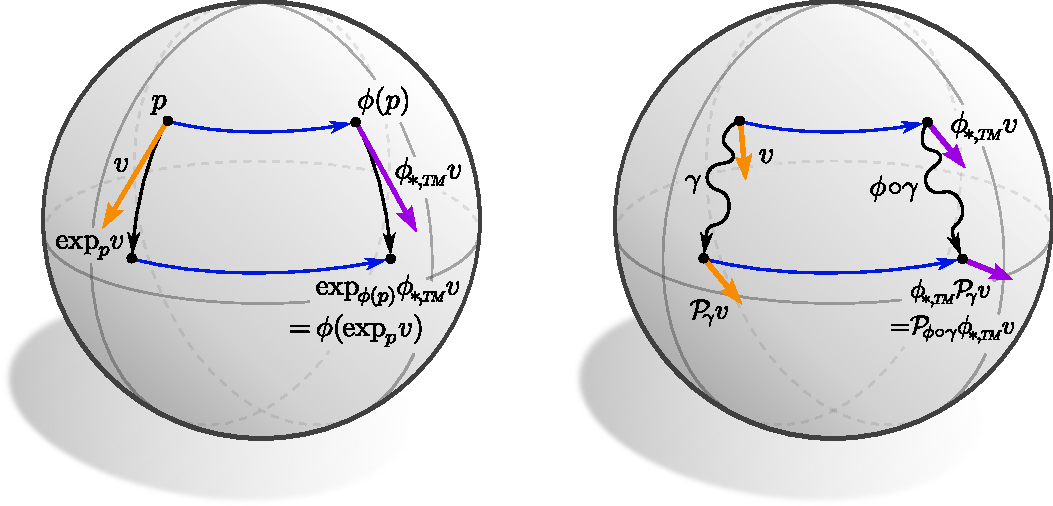
\includegraphics[width=.9\columnwidth]{figures/isometry_exp_transport.pdf}
    \vspace*{1ex}
    \caption{\small
        \ \emph{Left:}
        Isometries commute with the exponential map, that is,
        $\exp_{\phi(p)} \circ\, \protect\dphiTM (v) \,=\, \phi \circ \exp_p(v)$
        for any vector $v\in \TpM$ and isometry $\phi\in \IsomM$.
        \ \emph{Right:}
        Isometries also commute with the Levi-Civita transport of tangent vectors and feature vectors, that is,
        $\protect\dphiA\! \circ \protect\PAgamma \ =\ 
        \mathcal{P}_{\mkern-4mu\overset{}{\protect\scalebox{.6}{$\!\A$}, \mkern1mu\phi\circ\gamma}}\!
        \circ \protect\dphiA$
        for arbitrary paths $\gamma:[0,1]\to M$ and isometries $\phi\in \IsomM$.
        If an alternative, $G$-compatible connection is used, we demand that the same commutativity property holds for them.
        The isometry-invariance of exponential maps and transporters allows $\GM$-convolutions to be equivariant under the action of isometries.
    }
    \label{fig:isom_exp_transport}
\end{figure}






\paragraph{Isometries and parallel transporters:}
The pushforward on the tangent bundle was in~\cite{gallier2019diffgeom1} further argued to commute with the corresponding Levi-Civita transporters, as visualized in Fig.~\ref{fig:isom_exp_transport} (right).
If an alternative, $G$-compatible connection is chosen to transport feature vectors, we \emph{demand} that it commutes with the action of isometries as well.
Since the transporters and the pushforwards on $\FM$, $\GM$ and $\A$ are induced from those on $\TM$, one can easily show that this property translates to them.
Specifically for the associated feature vector bundles this means that for arbitrary isometries $\phi \in \IsomGM$ and paths $\gamma$ we assume the relation
\begin{align}\label{eq:transport_isom_commutation}
    \dphiA\! \circ \PAgamma
    \ =\ 
    \mathcal{P}_{\mkern-4mu\overset{}{\protect\scalebox{.6}{$\!\A$}, \mkern1.5mu\phi \mkern1.5mu\circ\mkern1.5mu \gamma}}\!
    \circ \dphiA
\end{align}
to hold, such that the following diagram commutes:
\begin{equation}
\quad
\begin{tikzcd}[column sep=70pt, row sep=40, font=\normalsize]
    \A_{\gamma(0)}
        \arrow[r, "\dphiA"]
        \arrow[d, "\PAgamma"']
    &
    \A_{\phi \mkern1mu\circ\mkern1mu \gamma(0)}
        \arrow[d, "\mathcal{P}_{\mkern-4mu\overset{}{\protect\scalebox{.6}{$\!\A$}  \mkern-0mu,\phi \mkern1mu\circ\mkern1mu \gamma}}"]
    \\
    \A_{\gamma(1)}
        \arrow[r, "\dphiA"']
    &
    \A_{\phi \mkern1mu\circ\mkern1mu \gamma(1)}
\end{tikzcd}
\end{equation}






\paragraph{Isometries and transporter pullbacks of feature fields:}

Knowing the transformation laws of exponential maps and transporters under the action of isometries, we have everything at hand that is required to derive the transformation law of transporter pullbacks $\Expspf$ of feature fields~$f$:
\begin{thm}[Isometry action on transporter pullbacks of feature fields]
\label{thm:transporter_pullback_isometry_action}
    Let $f\in \Gamma(\A)$ be any feature field and let $\phi \in \IsomGM$ be any $G$-structure preserving isometry.
    Assume the feature vector transporters to commute with the action of $\IsomGM$, that is, that Eq.~\eqref{eq:transport_isom_commutation} holds
    (which is automatically guaranteed for the Levi-Civita connection).
    The transporter pullback (Def.~\ref{dfn:Expf_pullback_field}) of the pushforward field $\phi\rhd \!f$ (Def.~\ref{dfn:isometry_pushforward}) is then given by:
    \begin{align}\label{eq:transporter_pullback_isometry_commutativity}
        \Expsp (\phi \rhd f)
        \ =\ 
        \dphiAout \!\circ \big[\mkern-2mu \Expsphiinvpf \mkern1mu\big] \circ \dphiTM^{-1}
    \end{align}
\end{thm}
\begin{proof}
    We start by letting the right-hand side act on an arbitrary vector $v\in\TpM$ and work progressively to the left-hand side by using the properties derived in this section:
    \begin{alignat}{3}
         &\,\ \dphiAout \big[\mkern-2mu \Expsphiinvpf \mkern1mu\big] \, \dphiTM^{-1} (v) \\
        =&\,\ \dphiAout\, \mathcal{P}_{\mkern-5mu\overset{}{\protect\scalebox{.8}{$\!\Ain$},\protect\scalebox{.85}{$\mkern2mu\phiinv(p) \mkern-3mu\leftarrow\mkern-1mu \exp_{\phiinv(p)} \!\circ\mkern2mu \dphiTM^{-1}(v)$}}}
            \circ f \circ \exp_{\phiinv(p)} \mkern-2mu\circ\, \dphiTM^{-1} (v)
            \quad && \big( \text{\small transporter pullback, Def.~\ref{dfn:Expf_pullback_field} } \big) \notag\\
        =&\,\ \dphiAout\, \mathcal{P}_{\mkern-5mu\overset{}{\protect\scalebox{.8}{$\!\Ain$},\protect\scalebox{.85}{$\mkern2mu\phiinv(p) \mkern-3mu\leftarrow\mkern-1mu \phiinv\mkern-2mu \circ \exp_p (v)$}}}
            \circ f \circ \phiinv \circ \exp_p (v)
            \quad && \big( \text{\small isometry action on $\exp$, Eq.~\eqref{eq:exp_isom_commutation}} \big) \notag\\
        =&\,\ \mathcal{P}_{\mkern-5mu\overset{}{\protect\scalebox{.8}{$\!\Ain$},\protect\scalebox{.85}{$\mkern2mu p \mkern-3mu\leftarrow\mkern-1mu \exp_p (v)$}}}
            \circ \dphiAin \circ f \circ \phiinv \circ \exp_p (v)
            \quad && \big( \text{\small isometry action on $\mathcal{P}_{\mkern-5mu\overset{}{\protect\scalebox{.75}{$\!\Ain$}}}$, Eq.~\eqref{eq:transport_isom_commutation}} \big) \notag\\
        =&\,\ \mathcal{P}_{\mkern-5mu\overset{}{\protect\scalebox{.8}{$\!\Ain$},\protect\scalebox{.85}{$\mkern2mu p \mkern-3mu\leftarrow\mkern-1mu \exp_p (v)$}}}
            \circ (\phi \rhd f) \circ \exp_p (v)
            \quad && \big( \text{\small pushforward of fields, Eq.~\eqref{eq:pushforward_section_A}} \big) \notag\\
        =&\,\ \big[\mkern-2mu \Expsp (\phi \rhd f) \mkern1mu\big] (v)
            \quad && \big( \text{\small transporter pullback, Def.~\ref{dfn:Expf_pullback_field} } \big) \notag
    \end{alignat}
\end{proof}
Intuitively, this result just states that the transporter pullback of a pushforward field equals the pushforward of the original field's transporter pullback.
Relative to local trivializations, this pushforward can be interpreted as an isometry induced gauge transformation, which was stated in Eq.~\eqref{eq:transporter_pullback_pushforward_field}.
We will in the following assume that the $G$-compatible connection which is chosen to transport feature vectors will always be $\IsomGM$-invariant, and thus that Eq.~\eqref{eq:transporter_pullback_isometry_commutativity} holds.


That the transporter pullback and the isometry pushforward commute is a consequence of the commutativity of the exponential map and parallel transporter, in terms of which the transporter pullback is defined.
Note that general diffeomorphisms do not preserve the metric and thus the exponential map and the transporter pullback of feature fields.
Being based on these constructions, kernel field transforms and $\GM$-convolutions can only be isometry equivariant but not fully diffeomorphism equivariant.
